\chapter{Design}
\label{chap:design}
\section{System Architecture and Required Functionality}
\label{sec:system_arch_and_req}
\begin{figure}[H]
	\centering
	\label{fig:block_simp}
	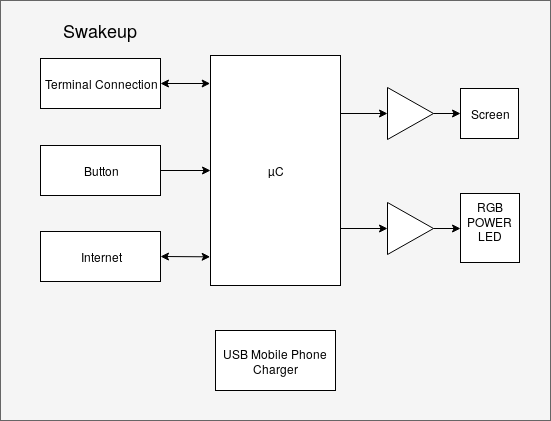
\includegraphics[width=0.6\textwidth]{../block/block_simplified.png}
	\caption{Simplified blockdiagram of Swakeup.}
\end{figure}
In fig. \ref{fig:block_simp} a simplified system architecture from an abstract
(e.g. customer) point of view is displayed. The heart of the system is a
microcontrolller. This microcontroller has to procide the necessary peripherals
and enough RAM and flash for the necessary funtionality, which has to be
implemented in software.  \newpar A terminal connection is crucial to transport
data to a computer. One needs this to do debugging and development. The idea is,
that a USB cbale can simply be plugged in and then the developer can start
working without additional complications.  \newpar A button is not only usefull
for the programmer to interact with the code to set the system to a certain
state, but it is also absolutely needed for deployment of the systems in the
real world.  Obviously, it should be extra convenient and simple for a sleepy
user to snooze (e.g. short button pressing) or to turn off the alarm (e.g. long
button pressing).  \newpar The idea of a IoT device is of course, that it is
connected to the internet, that is why a component has to be included into the
design to, which enables the system to receive a IP address. As the final
product will be standing most likely on a bedside table of the customer a wired
internet connection (e.g. Ethernet) does not make any sense. Instead a wireless
connection is more convenient (e.g. IEEE 802.11).  \newpar USB charging
circuitry i.e. a USB dedicated charging port has to be implemented to charge
phones with a current of at leas \SI{1.5}{A}.  \newpar As screen provides
information to the user, which goes beyond the current date and time (e.g.
weather, social media and email). It is reasonable, that this screen needs to be
powered somehow. Also the software developer or the user should have controll
over the screen brightness.  This means, that some time has to be invested in
the contruction of a powerful software-steerable screen driver.  \newpar To
light up a multi-color LED with a sufficient brightness to emulate a sunrise
circuitry has to be implemented to drive a high current. This current has to be
steerable in magnitude by the microcontroller to mix colors together according
to the RGB color model. 

\section{Design Choices}

% Please add the following required packages to your document preamble:
% \usepackage[normalem]{ulem}
% \useunder{\uline}{\ul}{}
\newcolumntype{L}[1]{>{\raggedright\let\newline\\\arraybackslash\hspace{0pt}}m{#1}}
\newcolumntype{C}[1]{>{\centering\let\newline\\\arraybackslash\hspace{0pt}}m{#1}}
\newcolumntype{R}[1]{>{\raggedleft\let\newline\\\arraybackslash\hspace{0pt}}m{#1}}
\begin{table}[H]
	\centering 
	\begin{tabular}{p{0.2\textwidth} p{0.2\textwidth} p{0.1\textwidth} 
		p{0.4\textwidth} } 
		\textbf{Block}           &
		\textbf{Component(s)}      &
		\textbf{Costs} 
		& \textbf{Justification of the
		Choice}
		\\\hline
		Terminal Connection      & SILICON LABS CP2102        & 24 SEK
		& Simple chip. Drivers for different operating systems are
		usually out-of-the-box available (plug and play). Available in
		QFN package.
		\\
		Internet                 & ESP8266                    & 25 SEK
		& ESP-E12 comes as ready to solder SMD module. No antenna design
		required. Easy connection to microcontroller via UART. Sming
		framework makes it easy to program chip in C++.
		\\
		USB Mobile Phone Charger & TS30012 and TPS2514        & 40 SEK
		& TS30012 is a relatively cheap chip to break down 20V to 5V and
		to provide up to 2A output current.  USB designated charging
		ports need signaling for different proprietary/open standards.
		TPS2514 is a quite nice chip to provide this signaling for
		different brands. \\
		RGB LED and Driver       & Custom Step-Down Converter & 20 SEK
		per Stage         & Fast, powerful LED driver built up with
		discrete components can be tailored to the requirements of the
		device and is therefore cheaper and more performant. Necessary
		feedback circuitry is also hard to find as COTS.
		\\
		Screen and Driver        & Custom Opamp Amplifier     & 30 SEK
		& One channel of the LM324 (four channel operational amplifier)
		was unused a simple circuit made it a cheap and easy-to-use DAC
		screen driver.    \\ 
		\hline
	\end{tabular}
	%\caption{My caption}
	\label{tab:design_choices}
\end{table}
